\documentclass[12pt]{exam}
\newcommand{\hwnumber}{3}
\newcommand{\hwname}{Images}
\newcommand{\duedate}{\formatdate{19}{9}{\YEAR} by \progDueTime} % day-month-year

%\newcommand{\hwcolor}{red}   % F18 S17 (upto F15)
%\newcommand{\hwcolor}{green} % S19 F17 S16
\newcommand{\hwcolor}{blue}  %  F19 S18 F16

\newcommand{\hwversion}{reflect-blur} % F19 F18 F17 F16 F15
%\newcommand{\hwversion}{rotate-mask}  % S19 S18 S17 S16

\usepackage{../misc/latex/edition}  % Course semester
\usepackage{../misc/latex/c0}       % Listings style for c0
\usepackage{amsmath}
\usepackage{enumerate}
\usepackage[normalem]{ulem}
\usepackage{verbatim}
\usepackage[left=1in, right=1in, top=1in, bottom=1in]{geometry}
\usepackage{graphicx}
\usepackage{hyperref}
\usepackage{tikz}     \usetikzlibrary{shapes}
\usepackage{fancybox}
\usepackage[all]{xy}
\usepackage{wrapfig}
\usepackage{fancyvrb}
\usepackage{datetime}
\usepackage{etoolbox}
\usepackage{calc}
\usepackage[nomessages]{fp}
\usepackage{import}  % Like input and include, but respects subdirectories

\newcommand{\defaultQuestionLocation}{questions}
\newcommand{\inputQuestion}[2][\defaultQuestionLocation/]{%
  \subimport{#1}{#2}
}
% Subdirectories of \defaultQuestionLocation containing code and pictures
\newcommand{\code}{code}
\newcommand{\img}{img}


%%% ic: frontmatter macros
\newcommand{\specialInstructions}{}
\newcommand{\HWNUMBER}
{\ifdefempty{\hwnumber}{__}{%
  \ifnumless{\hwnumber}{10}{0\hwnumber}{\hwnumber}}}
\newcommand{\hwtype}{Written Homework}

%%% ic: 'exam' tweaks
\renewcommand{\half}{.5} % Half points

\newcommand{\Question}[2][]
 {\ifstrempty{#1}
    {\question{\bf #2}}
    {\question[#1]{\bf #2}}
  \immediate\write\rubricfile{}%
  \immediate\write\rubricfile{Question \thequestiontitle:}%
  \immediate\write\rubricfile{==========}
 }

%%% ic: Support for editable PDF
% counter name (some viewers misbehave if always the same)
\newcounter{editable}
\newcommand{\nextField}{\addtocounter{editable}{1}q\arabic{editable}}
\newcommand{\NextField}
 {\makebox[0pt][r]{\scalebox{0.1}{\color{White}\nextField}}}

% Color of edit area
\newcommand{\editAreaColor}{red}
% Single line answer:   \editableLine[extra parameters (optional)]{line width}
\newcommand{\editableLine}[2][]
{\textcolor{\editAreaColor}{%
 \underline{\hspace*{-0.25em}%
 \raisebox{-0.5ex}{%
 \TextField[width=#2, borderwidth=0, #1]{\NextField}}}}%
}
% Single line answer for code:  \editableLine[extra parameters (optional)]{line width}
\newcommand{\editableCodeLine}[2][]
{\textcolor{\editAreaColor}{%
 \underline{%
 \TextField[width=#2, height=1.5ex, borderwidth=0, #1]{\NextField}}}}
% Multiline answer:  \editableLine[extra parameters (optional)]{box height}
\newcommand{\editableBox}[2][]
{\leavevmode\hspace*{-0.1em}%
\TextField[height=#2, width=\linewidth,
           multiline=true, borderwidth=0.1, bordercolor=\editAreaColor,
           #1]{\NextField}}

%%%%% Same answer format as exams
\renewcommand{\rmdefault}{ppl}
\renewcommand{\sfdefault}{phv}
\newcommand{\answerColor}{Blue}

\ifprintanswers
\newcommand{\answer}[2]{\makebox[#1][c]{\color{\answerColor}#2}}
\else
\newcommand{\answer}[2]{\makebox[#1][c]{}\makebox[0pt]{\phantom{|}}}
\fi
\newcommand{\uanswer}[2]{\underline{\answer{#1}{#2}}}


%%% Write rubric snippet.  Usage:
% \RUBRIC
% any multi-line text (including \, #, %, whatever)
% ENDRUBRIC
%% (ENDRUBRIC should be on a line by itself)
\makeatletter
\def\RUBRIC
 {%
  \begingroup
  \let\do\@makeother\dospecials
  \endlinechar=`\^^J
  \@tofile%
 }
\def\ENDRUBRIC{ENDRUBRIC}
\def\@tofile#1^^J{%
  \def\@test{#1}%
  \ifx\@test\ENDRUBRIC
    \immediate\write\rubricfile{}  % End with an empty line
    \expandafter\@firstoftwo
  \else
    \expandafter\@secondoftwo
  \fi
  {\endgroup}%
  {\toks@{#1}%
   \begingroup\endlinechar=\m@ne
   \everyeof{\noexpand}%
   \xdef\@temp{\scantokens\expandafter{\the\toks@}}%
   \endgroup
   \immediate\write\rubricfile{\@temp}%
   \@tofile}%
}
\makeatother

%% Displays tags for an exercise in 'answer' mode
\newcommand{\TAGS}[1]
{\ifprintanswers%
  \rule{0em}{0ex}%
  \marginpar{\footnotesize%
    \fcolorbox{black}{Gray!25}{%
      \parbox[t]{2cm}{\raggedright\textbf{TAGS:}\\#1}}}%
  \ignorespaces%
 \fi}%


%% Page layout
\pagestyle{headandfoot}

\headrule
\header{\textbf{\courseNumber{} \hwtype{} \hwnumber}}
       {}
       {\textbf{Page \thepage\ of \numpages}}
\footrule
\footer{}{}{\COPYRIGHT}

\renewcommand{\partlabel}{\textbf{\thequestion.\thepartno}}
%\renewcommand{\partlabel}{\textbf{Task \thepartno}}
\renewcommand{\subpartlabel}{\textbf{\thesubpart.}}
\renewcommand{\thepartno}{\arabic{partno}}
\renewcommand{\thesubpart}{\alph{subpart}}
\pointpoints{pt}{pts}
\pointformat{\raisebox{0ex}[\height][0pt]{\fcolorbox{black}{yellow}{\themarginpoints}}}
\bonuspointformat{\raisebox{0ex}[\height][0pt]{\fcolorbox{black}{red}{\themarginpoints}}}
\marginpointname{\points}
\pointsinmargin
%\boxedpoints

\setlength\answerlinelength{2in}
\setlength\answerskip{0.3in}

\newcommand{\mkWrittenTitle}[1]{#1}
\newcommand{\mkDueDate}[1]{#1}
\newcommand{\mkEvalSummary}[1]{#1}
\newcommand{\mkGradetable}[1]{#1}



% This fixes an issue with the exam package version 2.6 and after,
% where 'framed' has been renamed to 'examframed' to avoid a conflict.
\ifcsmacro{examframed}{%
\newenvironment{framed}
{\begin{examframed}}
{\end{examframed}}
}{}

\begin{document}
\hwTitle

\noindent
This programming assignment will have you using arrays to represent
and manipulate images.

\bigskip
\noindent
The code handout for this assignment is on \autolab{} and at
\begin{center}
\whereisthetgz{images-handout.tgz}
\end{center}
The file \lstinline'README.txt' in the code handout goes over the contents
of the handout and explains how to hand the assignment in.  There is
a FIVE (5) PENALTY-FREE HANDIN LIMIT, with the idea that for each task
you can test your code, hand in, and then fix any bugs found by autolab
while working on and testing the next task. Make sure to leave enough
submissions to work on the optional Task 5, if you wish to do that.
Every additional handin will incur a small (5\%) penalty (even if
using a late day).

\paragraph{Style Grading:}
With this assignment, we will begin to emphasize \emph{programming
  style} more heavily. We will actually be looking at your code and
evaluating it based on the criteria outlined at
\url{http://cs.cmu.edu/~15122/misc/styleguide.pdf}. We will make
comments on your code via Autolab, and will assign an overall passing
or failing style grade. A failing style grade will be temporarily
represented as a score of -15 points.  This -15 will be reset to 0
once you:
\begin{enumerate}
\itemsep=-3pt
\item%
  fix the style issues,
\item%
  see a member of the course staff during office hours \textbf{within
    5 days} after the grades are released, and
\item%
  briefly discuss the style issues and how they were addressed.
\end{enumerate}
We will evaluate your code for style in two ways. We will use
\lstinline'cc0' with the \lstinline'-w' flag that gives style warnings
--- code that raises warnings with this flag is almost certain to fail
style grading. Because the \lstinline'-w' flag does not check for good
variable names, appropriate comments, or appropriate use of the
functions defined in \lstinline'pixel.c0' and
\lstinline'imageutil.c0', these issues will be checked by hand.

\begin{task}[3]
\TAGS{correctness, loop-invariant, safety}
  In addition to using good style, be sure to include appropriate contracts,
  \requires{}, \ensures{}, and \loopinvariant{}. Your annotations should at
  least be sufficient to ensure that all your array accesses are safe, and
  part of your grade will be based on a visual inspection of this.
\end{task}

\section{Image manipulation}

The programming problems you have for this assignment deal with
manipulating images. An image will be stored in a one-dimensional
array of pixels. (The C0 image library assumes the ARGB implementation
of pixels that you wrote last week.) Pixels are stored in the array
row by row, left to right starting at the top left of the image. For
example, if a $5 \times 5$ image has the following pixel ``values'':
$$
\begin{array}{ccccc}
a & b & c & d & e \\
f & g & h & i & j \\
k & l & m & n & o \\
p & q & r & s & t \\
u & v & w & x & y \\
\end{array}
$$
then these values would be stored in the array in this order:
$$
a\ b\ c\ d\ e\ f\ g\ h\ i\ j\ k\ l\ m\ n\ o\ p\ q\ r\ s\ t\ u\ v\ w\ x\ y
$$
In the $5 \times 5$ image, the pixel $i$ is in row 1, column 3 (rows
and columns are indexed starting with 0) but is stored in the one-dimensional
array at index 8. An image must have at least one pixel.

\begin{task}[4]
\TAGS{correctness, safety, testing}
  Complete the C0 file \lstinline'imageutil.c0'. As with the
  \lstinline'pixel.c0' implementation from last week, you must fill in
  the missing code and translate the English preconditions and
  postconditions into \requires{} and \ensures{} statements.
\end{task}

We do not require you to hand in an \lstinline'images-test.c0' file
that tests your \emph{imageutil} implementation the way you tested
your \emph{pixel} implementation. It would be a good idea to write one
to test your own implementation, however!

%  We will compile your program as
% follows:
% \begin{quote}
% \begin{lstlisting}[language={[coin]C}]
% cc0 -d imageutil.c0 imageutil-main.c0
% \end{listing}
% \end{quote}
% using your \lstinline'imageutil.c0' file. Your code must compile using
% these instructions with files shown in the order given.
% We do not distribute a \lstinline|imageutil-main.c0| file; you can check
% that \lstinline|imageutil.c0| compiles using \lstinline|coin|. You are
% encouraged to write your own \lstinline|imageutil-main.c0| file that tests
% \lstinline'imageutil.c0'.  Do NOT include a main function in your
% \lstinline'imageutil.c0' file.

\section{Image Transformations}

The rest of this assignment involves implementing the core part of a
series of image transformations. Each function you write will take an
array representation of the input image and return an array
representation of the output image. These functions should {\it not}
be destructive: you should make your changes in a copy of the array,
and not make any changes to the original array. Your implementations
should be relatively efficient, meaning both that they should have a
reasonable big-O running time and that they should take at most a few
seconds to run on our example images.

Remember that your code should have appropriate preconditions and
postconditions. It is always a precondition that the given width and height
are a valid image size that matches the length of the pixel array passed to
the function. It is always a postcondition that the returned array is a
different array from the one that was passed in, and that this resulting array
has the correct length.

In order to pass style grading, you will be expected to use functions
from the \emph{pixel} interface (the type \lstinline'pixel_t' and
functions \lstinline'get_red', \lstinline'get_green',
\lstinline'get_blue', \lstinline'get_alpha', and
\lstinline'make_pixel') and the \emph{imageutil} interface (the
functions \lstinline'is_valid_imagesize', \lstinline'get_row',
\lstinline'get_column', \lstinline'is_valid_pixel',
\lstinline'get_index') in the next two tasks.  On Autolab, we will
compile your code for tasks 2 and 3 against \emph{our} implementation
of the \emph{pixel} and the \emph{imageutil} interfaces, so you cannot add
new functions to these interfaces.


\paragraph{Testing.}
You should use the provided \lstinline'*-main.c0' files to help you test
your code. The use of these files is described in the
\lstinline'README.txt' in the code handout.

For this assignment, we are providing a program,
\lstinline'imagediff', to help you compare your output images to the
sample images in the handout, optionally saving an image that shows
you exactly where the two images differ. It is in the course directory
on \lstinline'afs', so it is available on any cluster machine or when you
are connected via ssh. For example:
\begin{lstlisting}[language={[coin]C}]
% imagediff -i images/sample.png -j images/my-image.png -o images/diff.png
\end{lstlisting}
This command compares the image \lstinline'images/sample.png' and
\lstinline'images/my-image.png' and creates a visual representation of the
difference in \lstinline'images/diff.png'.


\input{remove-\hwcolor}


\ifdefstring{\hwversion}{rotate-mask}{
\clearpage\subsection{Rotation Effect}
\label{sect:rotate}

In this task, you will create a rotation effect on an image.  The
core of this transformation is this function:
\begin{quote}
\begin{lstlisting}
pixel_t[] rotate(pixel_t[] pixels, int width, int height)
\end{lstlisting}
\end{quote}
The returned array should be the array representation of the
duplicated and rotated image.  An example of this transformation is given in
Figure~\ref{fig:carnegie-rotate}.

Your task here is to implement a function that takes as input an image
of size $w \times h$ and creates a ``rotation'' image of size $(w+h)
\times (w+h)$ that contains the same image repeated four times, the top
right image containing the original image, the top left containing the
original image rotated 90 degrees counterclockwise, the bottom left
containing the original image rotated 180 degrees, and the bottom
right containing the original image rotated 90 degrees clockwise.

The original image must have the same width and height in order to do the
``rotation'' effect, i.e., $w=h$. If the supplied image is not ``square''
(i.e., its width does not equal its height) or does not match the size given
by the given width and height, your function should abort with a precondition
failure when compiled and run with the \lstinline'-d' flag.

\begin{figure}
\centering
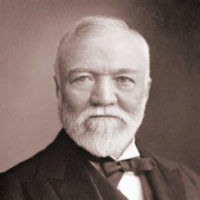
\includegraphics[scale=0.475]{\img/carnegie.png}
%\\[8em]
\quad\quad
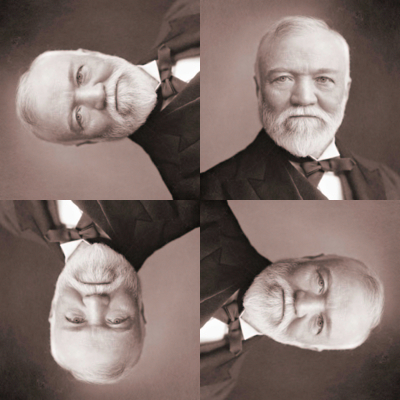
\includegraphics[scale=0.5]{\img/carnegie-rotate.png}
\caption{Original image (left); Image after ``rotation effect''}
\label{fig:carnegie-rotate}
\end{figure}

\begin{task}[8]
\TAGS{array, correctness, safety, testing}
  Create a C0 file \lstinline'rotate.c0' implementing a function
  \lstinline'rotate'.  You may include any auxiliary functions you
  need in the same file, but you should not include a
  \lstinline'main()' function.
\end{task}

You should look at \lstinline'README.txt' to see how to compile and run
this transformation against \lstinline'rotate-main.c0'.  You are also
strongly encouraged to write some test cases for your
programs in \lstinline'images-test.c0'.




%%% Local Variables:
%%% mode: latex
%%% TeX-master: "main"
%%% End:

\clearpage\subsection{Applying Masks to an Image}
\label{sect:mask}

In this problem, you will write a function that will apply a ``mask''
to an image. The core of this transformation is this function:
\begin{quote}
\begin{lstlisting}
int[] apply_mask(pixel_t[] pixels, int width, int height,
                 int[] mask, int maskwidth);
\end{lstlisting}
\end{quote}
The returned array should contain the results of running the mask
computation, a weighted sum, on each pixel in the input.
This is an array of \emph{integers}, not an array of pixels;
each integer in the returned array corresponds to a pixel in the
given image.

\paragraph{Masks}

In addition to an input image, we pass this transformation a
\emph{mask}, an $n \times n$ array of integers
representing \emph{weights}.  For our purposes, $n$ must be
odd. This means that the $n \times n$ array has a well defined center
--- the \emph{origin}. The weights in the mask can be arbitrary integers
--- positive, negative, or zero.

For each pixel in the input image, think of the mask as being placed
on top of the image so its origin is on the pixel we wish to
examine. The intensity value of each pixel under the mask is multiplied by
the corresponding value in the mask that covers it. These products are added
together.  Always use the original values for each pixel for each mask
calculation, not the new values you compute as you process the image.

\begin{figure}
  \begin{minipage}[c]{0.6\textwidth}\centering
    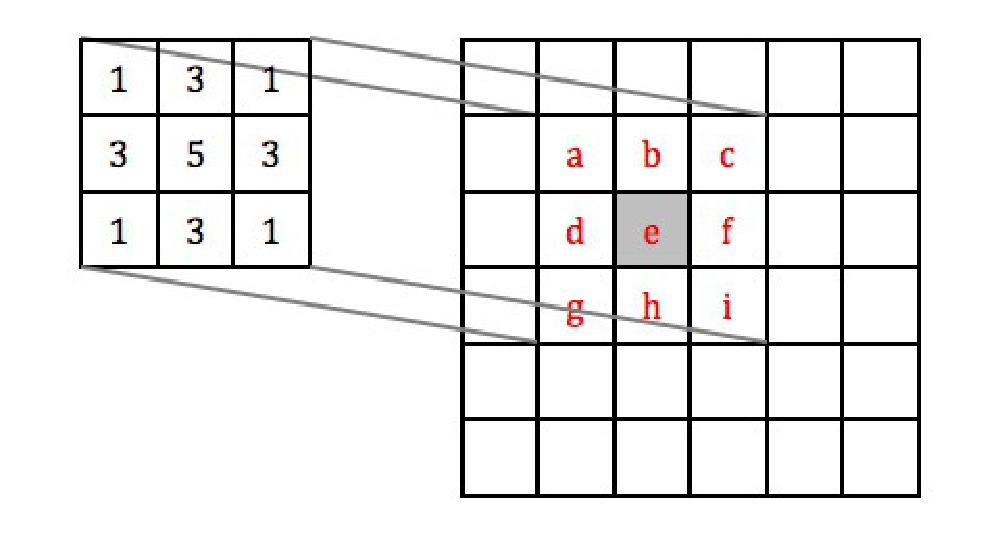
\includegraphics[scale=0.45]{\img/blurexample-eps-converted-to.pdf}
  \end{minipage}\hfill
  \begin{minipage}[c]{0.37\textwidth}
    \caption{Overlay the $3 \times 3$ mask over the image so it is centered on
      pixel $e$ to compute the new value for pixel $e$.}
    \label{fig:blur-example1}
  \end{minipage}
\end{figure}

\begin{figure}
  \begin{minipage}[c]{0.6\textwidth}\centering
    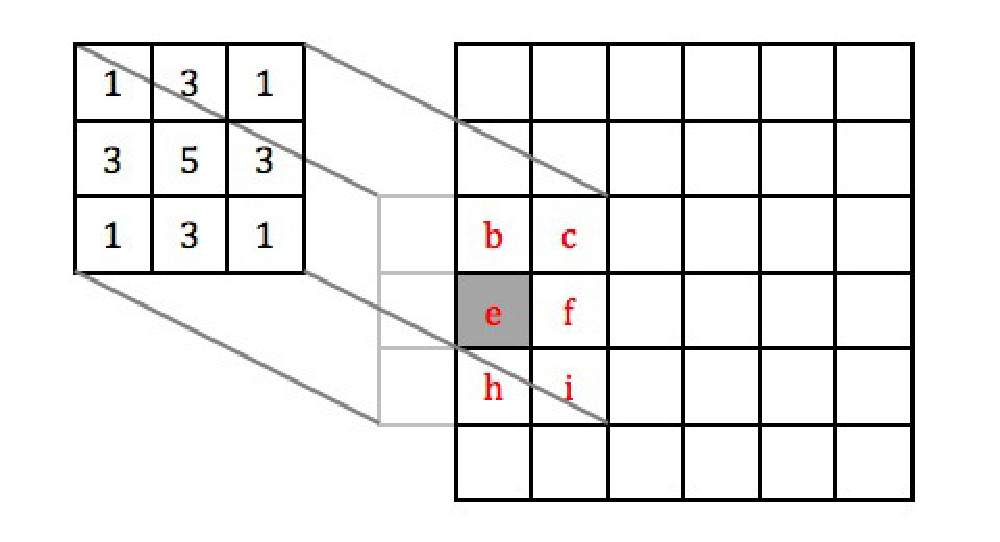
\includegraphics[scale=0.45]{\img/blurexample2-eps-converted-to.pdf}
%% The integer in index 18 of the returned array should be
%% \lstinline'3b + c + 5e + 3f + 3h + i'\\ where \lstinline'b' is the average intensity
%% of the pixel labeled \lstinline'b' and so on.
  \end{minipage}\hfill
  \begin{minipage}[c]{0.37\textwidth}
    \caption{If the mask hangs over the edge of the image, use only those mask
      values that cover the image in the weighted sum.}
    \label{fig:blur-example2}
  \end{minipage}
\end{figure}

For example, refer to Figure~\ref{fig:blur-example1}, which shows a $3
\times 3$ mask and an image that we want to perform the mask
computation on. Suppose we want to compute the result of the mask
computation for pixel \lstinline'e'. This result would be:
\begin{quote}
\begin{lstlisting}
a + 3b + c + 3d + 5e + 3f + g + 3h + i
\end{lstlisting}
\end{quote}
\pagebreak[4] Instead of doing this calculation for each channel
individually, use the average value of the red, green, and blue
channels --- we ignore the alpha channel. Going back to the example in
Figure~\ref{fig:blur-example1}, if the pixels \lstinline'a' and
\lstinline'e' are both given by $(a, r, g, b) = (255, 107, 9, 217)$,
then use $(107 + 9 + 217) / 3 = 111$ as the average intensity of those
pixels. If every other pixel in that figure is given by $(a, r, g, b)
= (15, 200, 120, 100)$ for an average intensity of $140$, then index
14 (which corresponds to pixel \lstinline'e' in
Figure~\ref{fig:blur-example1}) of the returned array should store
$2766$:
\begin{quote}
$111 + (3\times{}140) + 140 + (3\times{}140) + (5\times{}111) + (3\times{}140) + 140 + (3\times{}140) + 140 = 2766$
\end{quote}

Note that sometimes when you center the mask over a pixel you want to operate
on, the mask will hang over the edge of the image. In this case, compute the
weighted sum of only those pixels the mask covers. For the example shown in
Figure~\ref{fig:blur-example2}, the result stored in index 18 of the returned
array, which corresponds to pixel \lstinline'e', is given by
\begin{quote}
\begin{lstlisting}
3b + c + 5e + 3f + 3h + i
\end{lstlisting}
\end{quote}
where \lstinline'b' is the average intensity
of the pixel labeled \lstinline'b' and so on.


\begin{task}[10]
\TAGS{array, safety, testing}
  Create a C0 file \lstinline'mask.c0' implementing a function
  \lstinline'apply_mask'. You may include any auxiliary functions you
  need in the same file, but you should not include a
  \lstinline'main()' function.
\end{task}

You should look at \lstinline'README.txt' to see how to use this
transformation to perform a grayscale blur (\lstinline'maskblur-main.c0')
and edge detection algorithms (\lstinline'maskedge-main.c0'). The next
page talks a little bit about how these algorithms, especially edge
detection, work. You are also strongly encouraged to write some
test cases for your programs in file \lstinline'images-test.c0'.

\begin{figure}[bt]
\centering
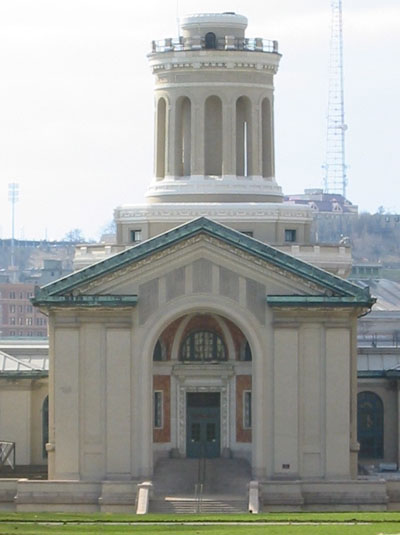
\includegraphics[scale=0.3]{\img/cmu.png}
\quad
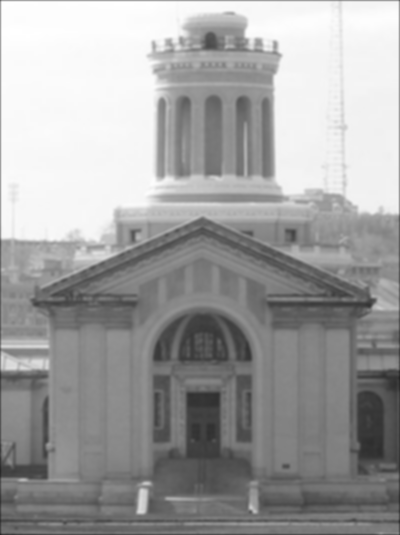
\includegraphics[scale=0.3]{\img/cmu-gaussian.png}
\quad
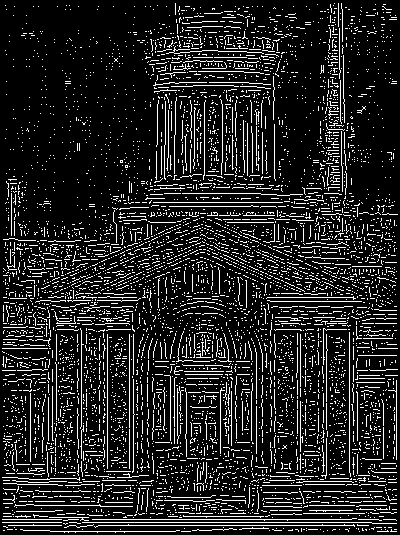
\includegraphics[scale=0.3]{\img/cmu-edge.png}
\caption{Hammerschlag Hall: original image (left), blurred with the mask
  (middle), and after running edge detection (right). See text for mask values.}
\label{fig:carnegie-blur}
\end{figure}

\clearpage
\subsubsection*{Applications}
\label{sect:applications}

The first main function you are given to test your code,
\lstinline'maskblur-main.c0', reads a mask from a text file, specified
by the \lstinline'-m' option. The mask is read in from the file and
passed along to \lstinline'apply_mask'. Then, the data returned from
\lstinline'apply_mask' is used to calculate new intensity values for
the pixels. This is done by summing all of the weights of the mask and
dividing by it. Note that this will cause the edge of the image to
have a lower intensity than it should, since we're not considering the
part of the mask that hangs off of the image, but this is an
acceptable simplification of the problem. Since we're allowing our
masks to have negative values, this creates the possible issue of
having an intensity greater than 255. If this is the case, the
intensities are modified appropriately --- for the blur masks, the
\lstinline'maskblur-main.c0' program will do division to get an
average intensity that is between 0 and 255.  Since we're returning
just one value instead of one per channel, this has the effect of
converting the image to grayscale.

One application of masks is blurring an image, which would be the
effect created by the examples shown in Figure~\ref{fig:blur-example1}
and Figure~\ref{fig:blur-example2}.

The other main function you are given to test your code,
\lstinline'maskedge-main.c0', implements an edge detection algorithm,
which is another application of masks.  The algorithm described here
is an implementation of Canny Edge Detection, using Sobel
operators. In this case, the function \lstinline'apply_mask' is called
three times. The first call will be to blur the image. For this
purpose, the following mask is used:
$$
\left[
\begin{array}{@{}rrrrr@{}}
   2 &  4 &  5 &  4 & 2
\\ 4 &  9 & 12 &  9 & 4
\\ 5 & 12 & 15 & 12 & 5
\\ 4 &  9 & 12 &  9 & 4
\\ 2 &  4 &  5 &  4 & 2
\end{array}
\right]
$$

After getting the resulting grayscale image, two more filters (the Sobel
operators) are applied to it. These filters determine the change in intensity,
which approximates the horizontal and vertical derivatives.
$$
\mathbf{G}_x =
\left[
\begin{array}{@{}rrr@{}}
   -1 & 0 & +1
\\ -2 & 0 & +2
\\ -1 & 0 & +1
\end{array}
\right]
\qquad
\text{and}
\qquad
\mathbf{G}_y =
\left[
\begin{array}{@{}rrr@{}}
   -1 & -2 & -1
\\  0 &  0 &  0
\\ +1 & +2 & +1
\end{array}
\right]
$$

After these two calls to \lstinline'apply_mask', the values obtained
are used to search for edges based on the magnitude and direction of
the change in intensity. An example of the final result is shown in
Figure~\ref{fig:carnegie-blur}.

You can even see the intermediate results of the X and Y filters individually by
trying:
\begin{quote}
\begin{lstlisting}[language={[coin]C}]
./maskblur -i images/cmu.png -m sobelX.txt -o images/cmu-edgeX.png
./maskblur -i images/cmu.png -m sobelY.txt -o images/cmu-edgeY.png
\end{lstlisting}
\end{quote}



%%% Local Variables:
%%% mode: latex
%%% TeX-master: "main"
%%% End:

}{}
\ifdefstring{\hwversion}{reflect-blur}{
\clearpage\subsection{Reflection Effect}
\label{sect:reflect}

In this problem, you will create a reflection effect on an image.
The core of this transformation is this function:
\begin{quote}
\begin{lstlisting}
pixel_t[] reflect(pixel_t[] pixels, int width, int height);
\end{lstlisting}
\end{quote}
Your task here is to implement a function that takes as input an image
of size $w \times h$ and creates an output image four times as large.
The top right quadrant of the output image will contain the original
image, the top left will contain the input image reflected across the
$y$-axis, the bottom right will contain the input image reflected across
the $x$-axis, and the bottom left will contain the input image reflected
across both axes.  A sample image is shown in
Figure~\ref{fig:carnegie-reflect}.

If the original image has size $w \times h$, the returned image should
have size $2w \times 2h$. If the supplied array does not exactly match
the size given by the width and height, your function should abort with
a precondition failure when compiled and run with the \lstinline'-d' flag.

\begin{figure}
\centering
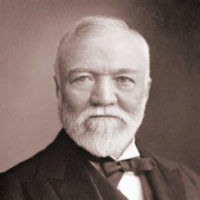
\includegraphics[scale=0.475]{\img/carnegie.png}
%\\[8em]
\quad\quad
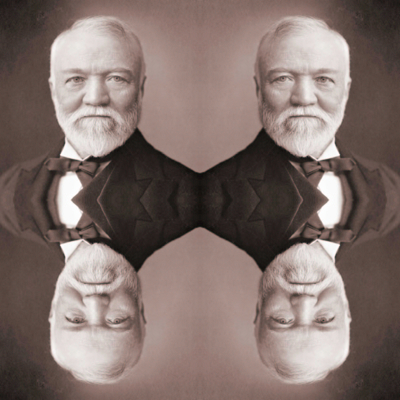
\includegraphics[scale=0.5]{\img/carnegie-reflect.png}
\caption{Original image (left); Image after ``reflection effect''}
\label{fig:carnegie-reflect}
\end{figure}

\vspace{0.1in}

\begin{task}[8]
\TAGS{array, correctness, safety, testing}
  Create a C0 file \lstinline'reflect.c0' implementing the function
  \lstinline'reflect'. You may include any auxiliary functions you need in the
  same file, but you should not include a \lstinline'main()' function.
\end{task}

You should look at \lstinline'README.txt' to see how to compile and run
this transformation using \lstinline'reflect-main.c0'. You are also
strongly encouraged to write some test cases for your
programs in \lstinline'images-test.c0'.


%%% Local Variables:
%%% mode: latex
%%% TeX-master: "main"
%%% End:

\clearpage\subsection{Blurring an Image}
\label{sect:blur}

In this task, you will write a function to blur an image. The core of this
transformation is this function:
\begin{quote}
\begin{lstlisting}
pixel_t[] blur(pixel_t[] pixels, int width, int height,
               int[] mask, int maskwidth)
\end{lstlisting}
\end{quote}
The returned array should be the representation of the blurred image.

\paragraph{Masks}
In addition to an input image, we pass the blur transformation a
\emph{mask}, an $n \times n$ array of non-negative integers
representing \emph{weights}.  For our purposes, $n$ must be odd. This
means that the $n \times n$ array has a well defined center --- the
\emph{origin}.  While weights in the mask can be 0 (but not negative),
the weight in the center position of the mask cannot be zero.

For each pixel in the input image, think of the mask as being placed
on top of the image so its origin is on the pixel we wish to
alter. The original intensity value of each pixel under the mask is
multiplied by the corresponding value in the mask that covers it.
These products are added together, and then we divide by the total of
the weights in the mask to get the intensity of the output pixel. Always
use the original (input) values for each pixel for each mask calculation, not
the output values you compute as you create the new image.


\begin{figure}
  \begin{minipage}[c]{0.6\textwidth}\centering
    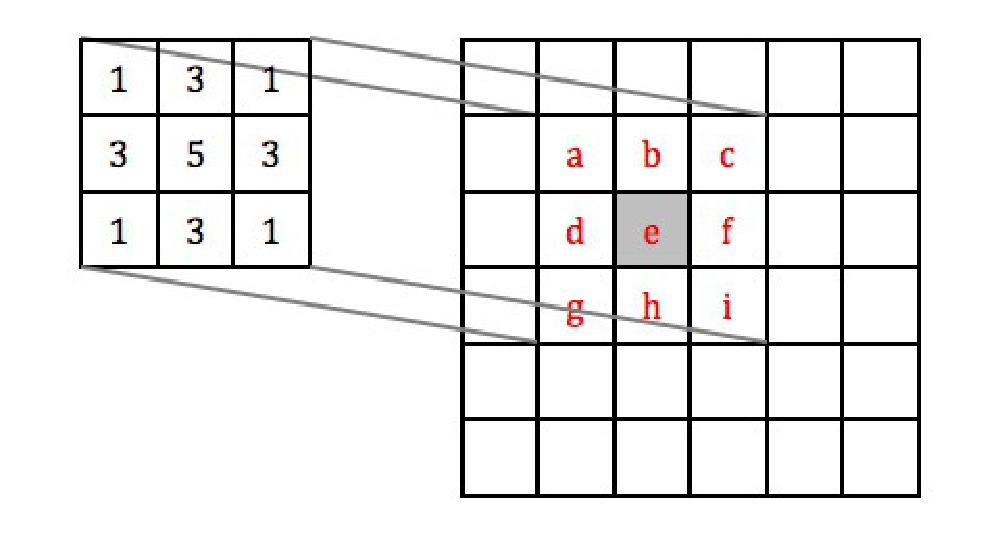
\includegraphics[scale=0.45]{\img/blurexample-eps-converted-to.pdf}
  \end{minipage}\hfill
  \begin{minipage}[c]{0.37\textwidth}
    \caption{Overlay the $3 \times 3$ mask over the image so it is centered on
      pixel $e$ to compute the new value for pixel $e$.}
    \label{fig:blur-exampleA}
  \end{minipage}
\end{figure}

\begin{figure}
  \begin{minipage}[c]{0.6\textwidth}\centering
    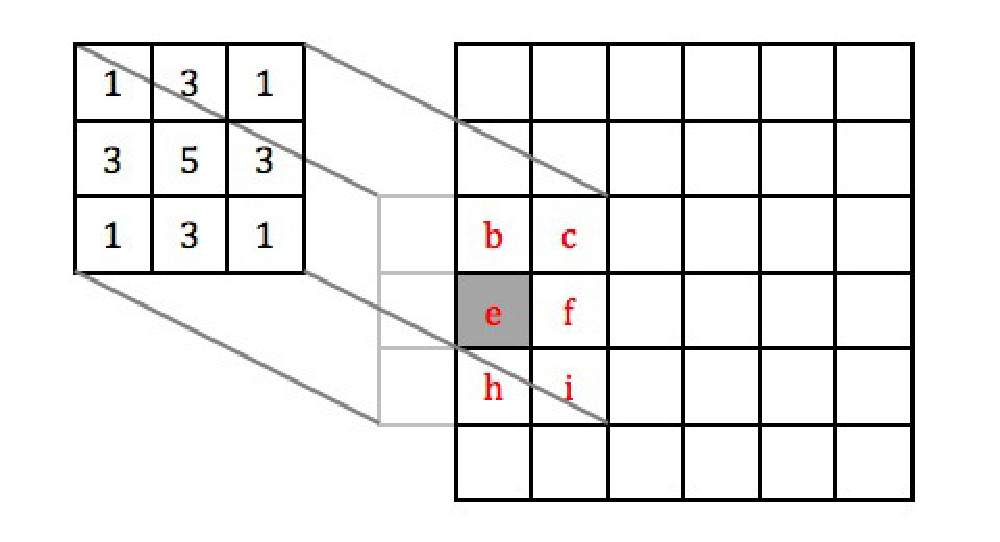
\includegraphics[scale=0.45]{\img/blurexample2-eps-converted-to.pdf}
%% The integer in index 18 of the returned array should be
%% \lstinline'3b + c + 5e + 3f + 3h + i'\\ where \lstinline'b' is the average intensity
%% of the pixel labeled \lstinline'b' and so on.
  \end{minipage}\hfill
  \begin{minipage}[c]{0.37\textwidth}
    \caption{If the mask hangs over the edge of the image, use only those mask
      values that cover the image in the weighted sum.}
    \label{fig:blur-exampleB}
  \end{minipage}
\end{figure}
% \begin{figure}[t]
%   \begin{minipage}[c]{0.67\textwidth}\centering
%     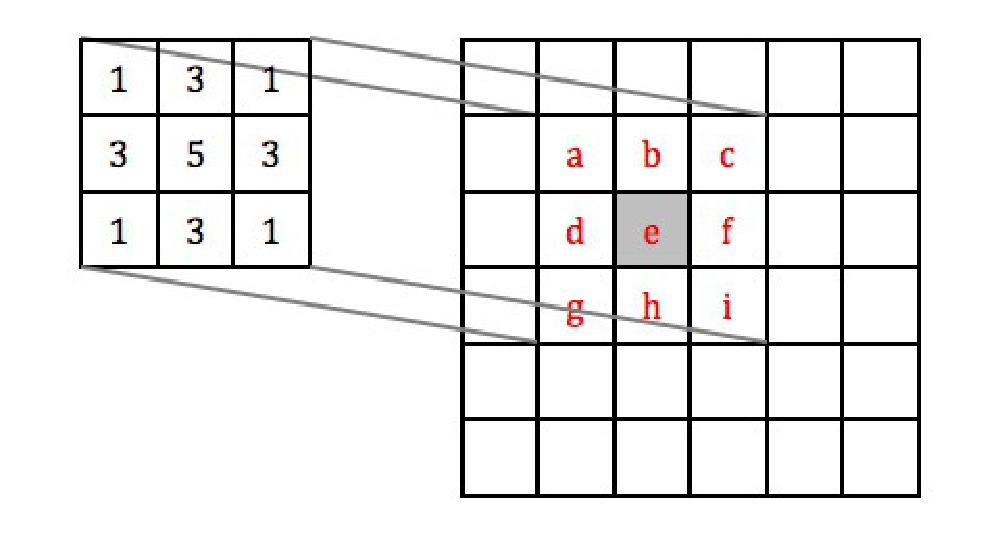
\includegraphics[scale=0.45]{\img/blurexample-eps-converted-to.pdf}
%   \end{minipage}\hfill
%   \begin{minipage}[c]{0.3\textwidth}
%     \caption{Overlay the $3 \times 3$ mask over the image so it is centered on
%       pixel $e$ to compute the output value corresponding to pixel $e$.}
%     \label{fig:blur-example}
%   \end{minipage}
% \end{figure}

For example, refer to Figure~\ref{fig:blur-exampleA}, which shows a $3 \times
3$ mask and an image that we want to blur. Suppose we want to compute the
output intensity value based on pixel \lstinline'e'.  Imagine overlaying the
mask so its center position is on \lstinline'e'.  We would compute the output
intensity for \lstinline'e' as:

\begin{quote}
\begin{lstlisting}
(a + 3b + c + 3d + 5e + 3f + g + 3h + i)  / 21
\end{lstlisting}
\end{quote}
This calculation is done three times for each pixel, once for its red channel,
once for its green channel, and once for its blue channel. Do not apply the
transformation to the alpha channel of the pixel.

% \begin{figure}
%   \begin{minipage}[c]{0.67\textwidth}\centering
%     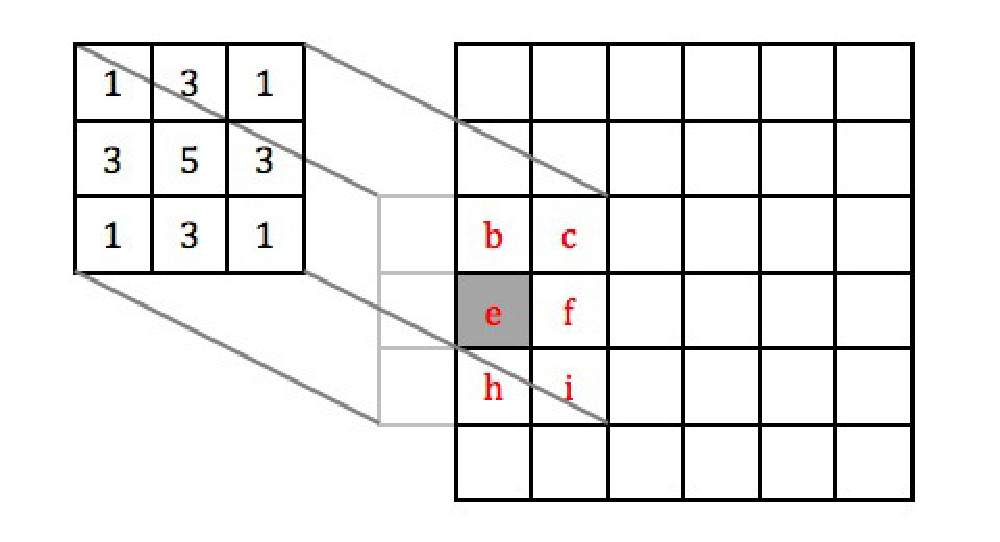
\includegraphics[scale=0.45]{\img/blurexample2-eps-converted-to.pdf}
%   \end{minipage}\hfill
%   \begin{minipage}[c]{0.3\textwidth}
%     \caption{If the mask hangs over the edge of the image, use only those mask
%       values that cover the image in the weighted sum.}
%     \label{fig:blur-example2}
%   \end{minipage}
% \end{figure}


Note that sometimes when you center the mask over a pixel you want to
blur, the mask will hang over the edge of the image. In this case,
compute the weighted sum of only those pixels the mask covers. In
these cases, you must divide by the sum of only those weights that you
use from the mask. For the example shown in
Figure~\ref{fig:blur-exampleB}, the output intensity for the pixel
\lstinline'e' is given by:
\begin{quote}
\begin{lstlisting}
(3b + c + 5e + 3f + 3h + i)  / 16
\end{lstlisting}
\end{quote}

\begin{figure}[b]
\centering

\includegraphics[scale=1]{\img/scs.png}
\quad

\includegraphics[scale=1]{\img/scs-blur-slightly.png}
\quad

\includegraphics[scale=1]{\img/scs-blur.png}
\caption{The SCS Dragon: original image (left), blurred slightly with
  a $3 \times 3$ mask (middle), and blurred with a $5 \times 5$ mask
  (right). See text for mask values.}
\label{fig:carnegie-blur}
\end{figure}


Figure~\ref{fig:carnegie-blur} shows a sample image blurred using the
following masks, which are given in the handout as
\lstinline'blur-slightly-mask.txt' and \lstinline'blur-mask.txt',
respectively:
\begin{verbatim}
         1 3 1          1 2 3 2 1
         3 5 3          2 3 4 3 2
         1 3 1          3 4 5 4 3
                        2 3 4 3 2
                        1 2 3 2 1
\end{verbatim}

The \lstinline'mask' passed to the function must have width $n \times
n$, where $n$ is given by the argument \lstinline'maskwidth'.  If the
supplied image does not match the size given by \lstinline'width' and
\lstinline'height', or if the mask is not a square matching the size
given by \lstinline'maskwidth', or if \lstinline'maskwidth' is not
odd, or if the mask contains negative integers or a zero at the
origin, your program should abort with a precondition failure when
compiled and run with the \lstinline'-d' flag.

\begin{task}[10]
\TAGS{array, safety, testing}
Create a C0 file \lstinline'blur.c0' implementing a function
\lstinline'blur'. You may include any auxiliary functions you need in the
same file, but you should not include a \lstinline'main()' function.
\end{task}

You should look at \lstinline'README.txt' to see how to compile and run
this transformation against \lstinline'blur-main.c0'. You are also strongly
encouraged to write some test cases for your programs in a
file \lstinline'images-test.c0'.



%%% Local Variables:
%%% mode: latex
%%% TeX-master: "main"
%%% End:

}{}

\clearpage
\subsection{Your own image processing algorithm (Optional)}
\label{sect:prize}

In this task, you will perform an image manipulation of your choice.
The core of this transformation are three functions:
\begin{quote}
\begin{lstlisting}
int result_width(int width, int height)
int result_height(int width, int height)
pixel_t[] manipulate(pixel_t[] pixels, int width, int height)
\end{lstlisting}
\end{quote}
If \lstinline'I' is the representation of an image with width
\lstinline'w' and height \lstinline'h', then the result of calling
\lstinline'manipulate(I,w,h)' should the representation of image of
width \lstinline'result_width(w,h)' and height
\lstinline'result_height(w,h)'.

\begin{ectask}
\TAGS{array, safety}
  Create a C0 file \lstinline'manipulate.c0' implementing the three
  functions described above: \lstinline'result_width',
  \lstinline'result_height', and \lstinline'manipulate'. You may
  include any auxiliary functions you need in the same file, but you
  should not include a \lstinline'main()' function. You may not add
  arguments to \lstinline'manipulate', but you can write a separate
  function \lstinline'my_manipulate' (or whatever) and then call your
  function from the \lstinline'manipulate' function with some specific
  arguments.
\end{ectask}

You should look at \lstinline'README.txt' to see how to compile and run
this transformation against \lstinline'manipulate-main.c0'.

If you choose to do this task, be creative! Submissions will be
displayed on the Autolab scoreboard and we will highlight exemplary
submissions.
%To include your image in the scoreboard,
%use the \lstinline|handin| script and include the file \lstinline'output.png'
%-- if you don't include \lstinline'output.png', we'll use
%\texttt'g5.png'.
%
If you include a (small!) file \lstinline'manipulate.png',
we'll run your transformation against that image; otherwise
we'll run your transformation on \lstinline'g5.png'.

\begin{figure}[h]
\begin{center}
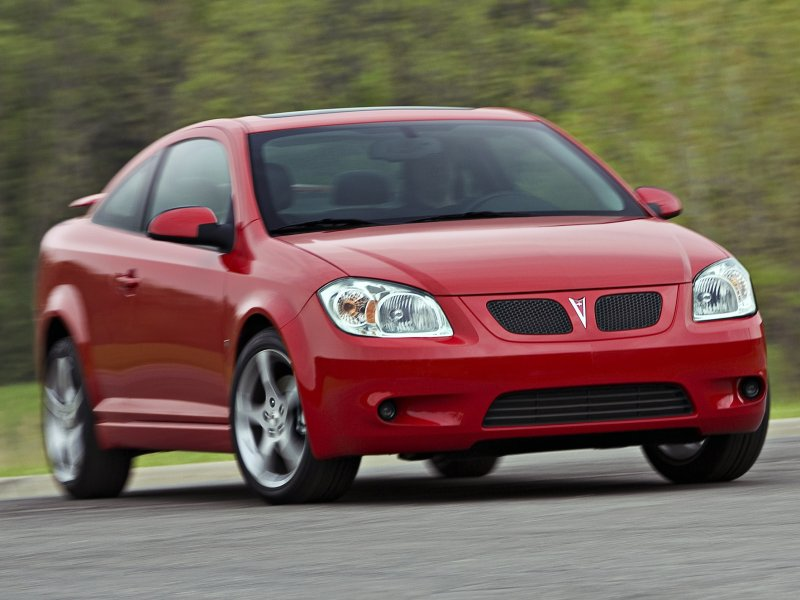
\includegraphics[scale=0.3]{\img/g5.png}
\end{center}
\caption{Manipulate me!}
\end{figure}


%%% Local Variables:
%%% mode: latex
%%% TeX-master: "main"
%%% End:


%% Unused
%\subsection{Selectively Inverting an Image}
\label{sect:invert}

You may be familiar with the ``invert colors'' or ``photo negative''
effect commonly available in image editors. In this problem, we will
invert the colors of only a part of an image. The part that we choose
to invert will be based on a target color and a tolerance level. You
can see an example in Figure~\ref{fig:g5_invert}.

\begin{figure}[h]
\centering
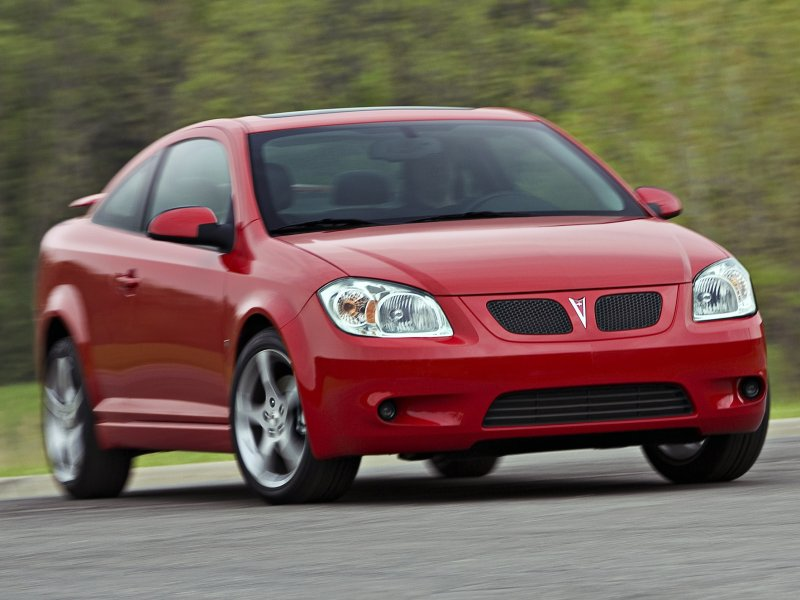
\includegraphics[scale=0.15]{\img/g5.png}
\quad
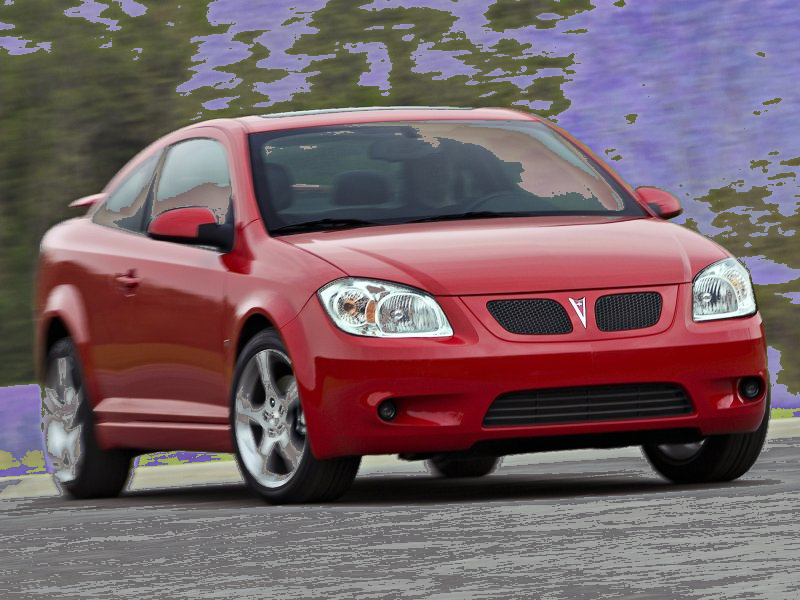
\includegraphics[scale=0.15]{\img/g5-invert1.png}
\quad
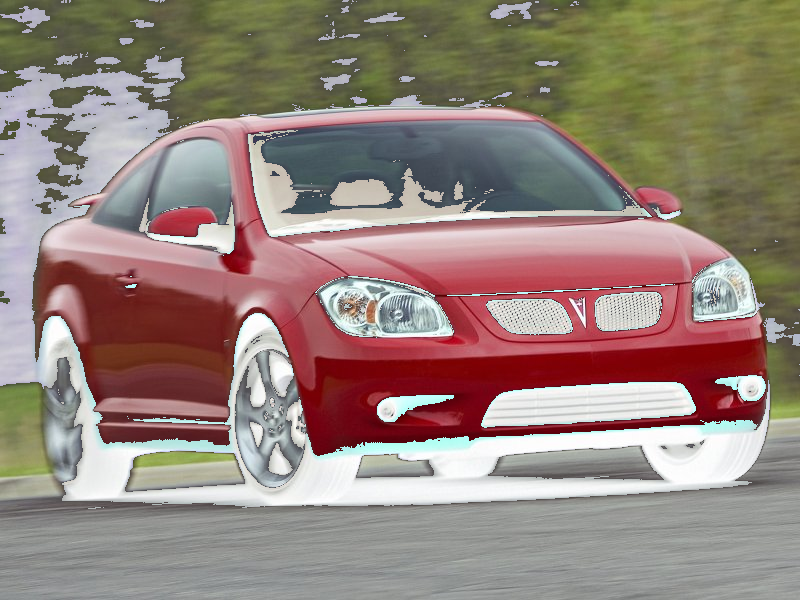
\includegraphics[scale=0.15]{\img/g5-invert2.png}
\caption{A sporty coupe with no inversion (left); partial
  inversion, color=\lstinline'0xffcf0000', tolerance=100 (middle);
  and full inversion, color=\lstinline'0xffcf0000', tolerance=255 (right).}
\label{fig:g5_invert}
\end{figure}
Given an ordinary image of size $w \times h$ along with a target color
and a tolerance, examine each pixel.  If the difference between the
starting pixel and the target color is less than or equal to the
tolerance for the red, green, and blue channels, then that pixel
should be inverted. You should not look at the alpha value.  The
tolerance will be specified as an integer between 0 and
255.  Essentially, if the target color is close enough to the color of
a particular pixel, that pixel should be inverted.  By inverting, we
mean flipping each bit. For example, suppose the color components for
a pixel are given by the bytes:

\begin{quote}
\renewcommand{\arraystretch}{1.2}
\begin{tabular}{l|lll}
   Color   & Red                  & Green                & Blue
\\\hline
   Binary  & \lstinline'01111101' & \lstinline'10100001' & \lstinline'10010111'
\\ Decimal & \lstinline'125'      & \lstinline'161'      & \lstinline'151'
\\ Hex     & \lstinline'0x7d'     & \lstinline'0xa1'     & \lstinline'0x97'
\end{tabular}
\end{quote}

And our target color is:
\begin{quote}
\renewcommand{\arraystretch}{1.2}
\begin{tabular}{l|lll}
   Color   & Red                   & Green                & Blue
\\\hline
   Decimal & \lstinline'143'       & \lstinline'178'      & \lstinline'158'
\\ Hex     & \lstinline'0x8f'      & \lstinline'0xb5'     & \lstinline'0x9e'
\end{tabular}
\end{quote}
If our tolerance is 20, then we have a match and should invert the pixel to the
following value:
\begin{quote}
\renewcommand{\arraystretch}{1.2}
\begin{tabular}{l|lll}
   Color   & Red                  & Green                & Blue
\\\hline
   Binary  & \lstinline'10000010' & \lstinline'01011110' & \lstinline'01101000'
\\ Decimal & \lstinline'130'      & \lstinline'94'       & \lstinline'104'
\\ Hex     & \lstinline'0x82'     & \lstinline'0x5e'     & \lstinline'0x68'
\end{tabular}
\end{quote}
Note that an image processed with a tolerance of 0 will only invert an exact
match and a tolerance of 255 will invert the entire image.
For each pixel, do not change its alpha component.

\vspace{0.1in}

\begin{task}[4]
\TAGS{array, correctness, safety, testing}
In the C0 file \lstinline'invert.c0', complete the \lstinline'invert'
function:
\begin{lstlisting}
pixel_t[] invert(pixel_t[] pixels, int width, int height,
                 int color, int tolerance);
\end{lstlisting}
This function should implement the algorithm described above, given an
array \lstinline'pixels' representing an image of width
\lstinline'width' and height \lstinline'height' using a target color
of \lstinline'color' and a tolerance of \lstinline'tolerance'. The
returned array should be the representation of the image after
inversion has occurred. It should \textbf{not} be destructive --- that
is, you should make your changes in a copy of the array, and not in
the original array.  You may include any auxiliary functions you need
in the same file, but you should not include a \lstinline'main()'
function. If the supplied tolerance level is out of range or if
\lstinline'width' and \lstinline'height' do not agree with the size of
the array \lstinline'pixels', your function should abort with an
annotation failure when run with the -d flag.
\end{task}

We will compile your program as follows:
\begin{lstlisting}[language={[coin]C}]
% cc0 -d imageutil.c0 invert.c0 invert-main.c0 -o invert
\end{lstlisting}
using your \lstinline'imageutil.c0' and \lstinline'invert.c0' files.
Your code must compile using these instructions with files shown in the order
given. Do NOT include a main function in your \lstinline'invert.c0' file.

After compiling, here is an example of how to call your program:
\begin{lstlisting}[language={[coin]C}]
% ./invert -i images/g5.png -o images/g5-invert.png -c 0xffcf0000 -t 100
\end{lstlisting}
Note that the target color is specified in hexadecimal, beginning with ``0x''.



%%% Local Variables:
%%% mode: latex
%%% TeX-master: "main"
%%% End:

%\subsection{Quantization of an Image}
\label{sect:quantize}

In this problem, you will implement a function that achieves a
quantization effect on an image.  Quantization reduces the total
number of colors used in an image.  You can see an example in
Figure~\ref{fig:g5_quantize}.

\begin{figure}
\centering
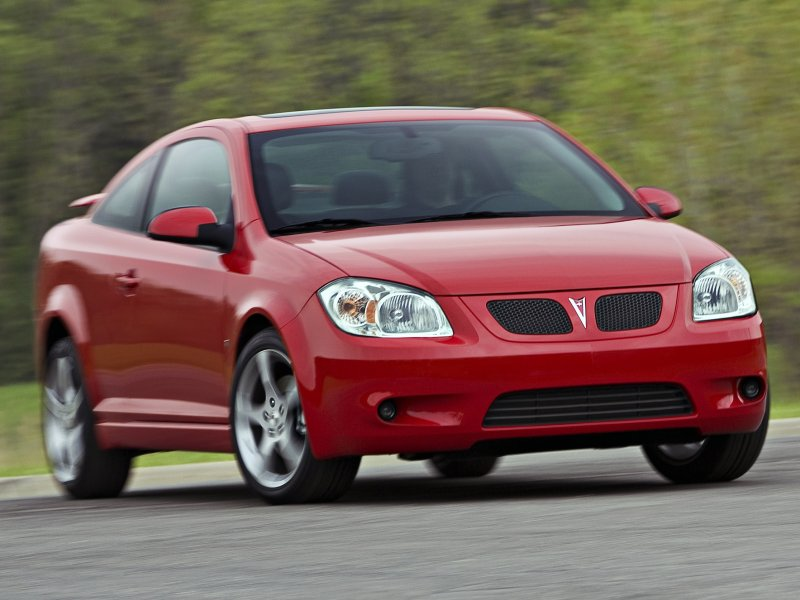
\includegraphics[scale=0.2]{\img/g5-quantize0.png}
\quad
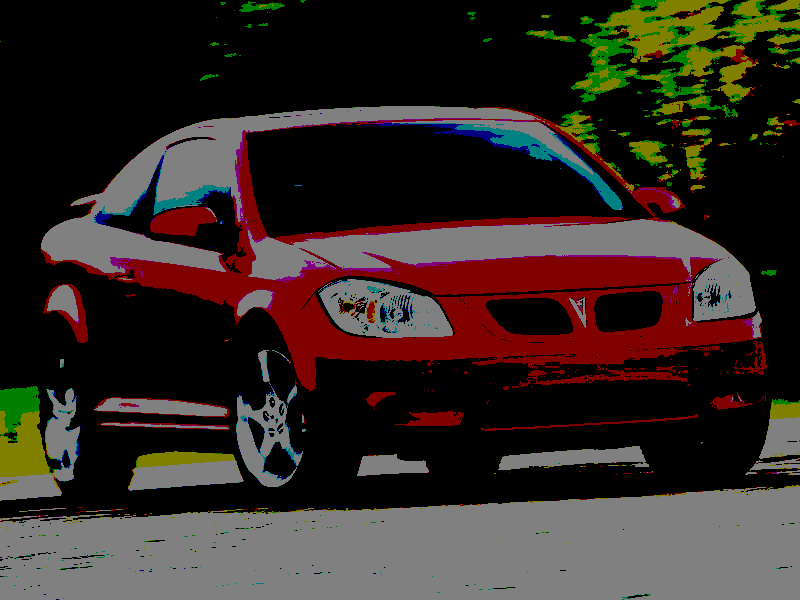
\includegraphics[scale=0.2]{\img/g5-quantize7.png}
\caption{A sporty coupe with quantization level 0 (left) and
level 7 (right).}
\label{fig:g5_quantize}
\end{figure}

Given an ordinary image of size $w \times h$ and a quantization level
$q$ between 0 and 7, inclusive, for each pixel in the image, take each
color component (red, green and blue) and clear the lowest $q$ bits.
For example, suppose the color components for a pixel are given by the
bytes
\begin{quote}
\renewcommand{\arraystretch}{1.2}
\begin{tabular}{lll}
   Red                  & Green                & Blue
\\\hline
   \lstinline'01101011' & \lstinline'10111110' & \lstinline'11010111'
\end{tabular}
\end{quote}
If the quantization level is 5, then the resulting pixel should have
the following color components (note how the lower 5 bits are all cleared to 0):
\begin{quote}
\renewcommand{\arraystretch}{1.2}
\begin{tabular}{lll}
   Red                  & Green                & Blue
\\\hline
   \lstinline'01100000' & \lstinline'10100000' & \lstinline'11000000'
\end{tabular}
\end{quote}
Note that an image processed with a quantization level of 0 should not change.
For each pixel, do not change its alpha component.




\vspace{0.1in}

\begin{task}[6]
\TAGS{array, correctness, safety, testing}
  Create a C0 file \lstinline'quantize.c0' with a function
  \lstinline'quantize' matching the following prototype:
\begin{lstlisting}
pixel_t[] quantize(pixel_t[] pixels, int width, int height, int q_level);
\end{lstlisting}
This function should implement the algorithm described above,
given an array \lstinline'pixels' representing an image of width
\lstinline'width' and height \lstinline'height' using a quantization
level \lstinline'q_level'.
\end{task}

We will compile your program as follows:
\begin{quote}
\begin{lstlisting}[language={[coin]C}]
% cc0 -d imageutil.c0 quantize.c0 quantize-main.c0 -o quantize
\end{lstlisting}
\end{quote}
using your \lstinline'imageutil.c0' and \lstinline'quantize.c0' files.
Your code must compile using these instructions with files shown in the order
given. Do NOT include a main function in your \lstinline'quantize.c0' file.
Sample usage is:
\begin{quote}
\begin{lstlisting}[language={[coin]C}]
% ./quantize -i images/g5.png -q 6
\end{lstlisting}
\end{quote}
Running this command should produce an image,
\lstinline'images/g5_quantize.png', that is identical to the file
\lstinline'images/g5-quantize6.png' distributed with the handout.


%%% Local Variables:
%%% mode: latex
%%% TeX-master: "main"
%%% End:


\end{document}
